\documentclass[11pt]{article}
\usepackage{fullpage}
\usepackage{graphicx}
\title{\textbf{Dual Screen} \\Passing fad or new way of life?}
\author{Miguel Vazquez}
\begin{document}
\maketitle
\begin{abstract}
With the growing integration of technology with our daily lives it seems only natural that we seek ways to enhance our interaction with it. One of those methods that have been emerging is the usage of two screens at once. This is not a new idea when it comes to computers and has a growing foothold into becoming standard. Within video games it has also begun to gain momentum. This paper analyzes the concept of two screens with both video games and computers.
\end{abstract}

\tableofcontents

\section{Introduction}
The main question this paper address is whether or not having more than one screen is simply a fad or if there is a legitimate use for multiple screens? In the future will multiple screens still be used, or will we revert back to having one screen. The idea of multiple screens is used in various aspects of life and currently has a following in its usage.
Multiscreen and Video games

\section{Research}
\subsection{Research on Multiple Monitor Computers}
Upon looking into the topic an experiment was found\cite{monitors} in which people were tested to see the type of monitor setup that was preferred. The experiment contained four different monitor setups. According to the results from the experiment the subjects preferred wider screens and preferred two screens over one. The experiment also found that with the widescreen two monitor setup the test subjects were able make the swiftest mouse movements of all other setups. A second study \cite{monitors2} showed that having more than one screen actually improved the productivity of the person working. However it does mention that there is a certain point where this no longer holds true. After a certain screen size and number the productivity no longer increases..

\subsection{Multiscreen and Video games}
In entertainment it seems to be a somewhat new concept still trying to get a foothold to become a standard default. Nintendo seems to be making its push with both its console the Wii U, which has a controller that contains the second screen, and its' hand-held systems the DS which has two  screens built in to it. The next generation system from Microsoft also boasts having the ability to connect to a tablet in order to allow the user more interaction. Whether it is a fad or not it seems that the video game industry wishes to try and invest in it. However this is not a new concept within the video game industry and has been pushd for a while by now. Nintendo gave its Gameboy Advance the ability to connect to the Gamecube in order to interact with it and allow for new ways to play.

\section{Methods}
\subsection{Explanation of Survey}
For this topic various people were asked on their opinion of a second screen. The questions asked were “What is your opinion on two monitors? Would you say it is a passing fad or here to stay?” The second question “With the Wii U sporting a controller that acts as a tablet and with the new Xbox trying to connect to tablets what is your opinion on a second screen with video games?” These questions were asked to the subjects they were also asked to explain their view. The results of the two surveys are shown in Figure ~\ref{monitor} and Figure ~\ref{Videogames} respectively

\begin{figure}[h!]
  \centering
    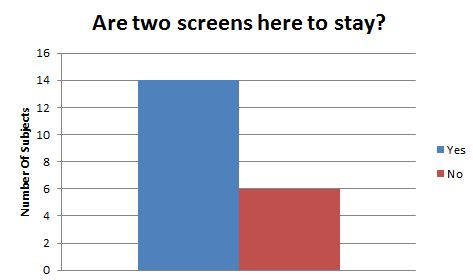
\includegraphics[width= 1\textwidth]{./Images/Monitors}
  \caption{Results on asking about two monitor video games}
 \label{monitor}
\end{figure}

\begin{figure}[h!]
  \centering
    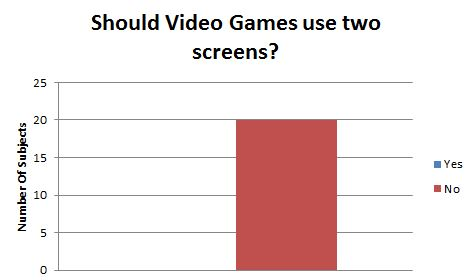
\includegraphics[width= 1\textwidth]{./Images/VideoGames}
  \caption{Results on asking about two screens with respect to video games}
 \label{Videogames}
\end{figure}

\section{Discussion}
\subsection{Research and Two Monitor Computers}
The research that was found with the two experiments stated that users tended to overlap their running programs less than they would with one monitor. This meant that users found themselves comfortable with leaving as many windows open as they wanted in order to change between each of them. The fact that they could see the actual windows meant that there was less error in selecting the correct window. Often when having multiple windows from the same software could lead to opening the appropriate window, especially when the proper window is buried under two or three different windows. The ability to have multiple windows open and each one being properly visible helps minimize this error. 

\subsection{Subjects and Two Monitor Computers}
Figure~\ref{monitor} shows the results of the survey when asking people their opinion on having two monitors on a computer. Most of the subjects that were asked for their opinion on have two monitors agreed that having two was better. The opinions of the matter are as follows. The usage of two screens will be further cemented as an industry standard once it is easier to connect to a second monitor and set it up. This opinion shows that there are some learnability problems with using a second monitor because it seems to be an intimidating feat to set up and can be a hassle at times. This person also stated that the next step in pushing for a second screen would be wireless technology allowing to connect to the monitors without having to worry about wiring. This would mean that the subject feels that there are certain errors that can be committed by them and will feel better with the technology once the amount of possible errors is lowered. Another subject stated that they have noticed that the usage of two monitors seems to be particularly big with jobs that involve scheduling or looking up information. This means that the retrieval and organization of data seems to be easier on two screens. Another subject provided a particularly interesting analogy on how they view having two monitors. They stated that when they work at home they have the option to work wherever they want but always find themselves at the kitchen table. The reason they particularly enjoy the kitchen table is because it allows them to have all their work and books related to the work spread out on the table. This allows for efficient referencing to the books while they work. They stated that this is the same concept they use with two monitors. They have all their software open at once and allow for a clear view of it at all times. This allows them to change between each efficiently and in some cases read information while keeping their work as the active window. The few people who felt that having two monitors is just a passing fad stated that they felt this way because they believed that a single widescreen would be more efficient. They stated that they felt the gap between the two screens would cause them to lose track of the mouse and with all of that space there would be difficulty to find the mouse once again.

\subsection{Research and Video Games}
As was stated the idea of having a second screen with video games has been around for a couple of years. The Gamecube allowed for connections with the Gameboy Advance which allowed for two screens. This was used with the 2004 game “The Legend of Zelda Four Swords Adventures.” This game allowed for up to four Gameboy Advances to be connected to the Gamecube and play. This concept allowed for the players to work individually without having to move with the rest of the player as was done with other games. The second screen remained blank whenever the player was in the “overworld” and was shown on the television screen. However once the player entered a home, cave, etc. the second screen would show the interior and the player. This allowed them to have their adventure without burdening the rest of players. These two screens allowed for the player to do actions that will affect the “overworld” and would allow them to directly see the results of their actions and how it affects the other players. This is simply one example of the two screen concept during this age of video games. When the DS first released it was evident that many of the developers were unsure of what to do with the second screen that was given to them. Many of the original games seemed to have just been made to be a single screen game with the second screen often having a simple placeholder such as a map, menu or player statistics. However as time passed some games began to take advantage of this screen allowing for the second screen to act as an extension to the single screen. This allowed for maps to span two screens and have boss battles that spanned two screens and cause some truly memorable moments. Now with the next generations approaching and wireless technology being at its level of sophistication it seems video game developers wish to push forward even more. The Wii U is allowing for the user interact with the game using the second screen with its touch pad capabilities. During E3 Microsoft stated they will allow for tablets to connect to the game and interact with the game. One of the example of this was with the reveal of the game Dead Rising 3, they plan on allowing for the tablet to mark locations of the game for missile strikes. This is something that could be done within the game and console on its own, however allowing for a tablet to directly mark and affect the gameplay adds for a new way to play.

\subsection{Subjects and Two Monitor Video Games}
Figure~\ref{Videogames} shows the results of surveying people on their opinions towards a second screen in video games. It seemed to be a unanimous disagreement on whether it is worthwhile addition to the way games are played. It seems that the subjects that were questioned did not like the idea of having to focus on two different screens. Some stated that two stationary screens next to each other would be acceptable. The complaints seem to have come with the Nintendo Wii U in mind. The idea was that having a second screen in that case is cause for problem due to the mobility of the second screen. The second screen in this case is the controller which acts as a tablet of sorts. The fact that this screen can be moved by the user causes for some variability of its location. The worry was that people would have to look at a different location every time to see what is happening in their game. The subjects stated they would find the second screen acceptable in this case if the screen was merely there to provide information like statistics and maps. If the second screen was meant to be an actual part of the in game action that would require the user to look at the second screen and act on it the users seemed to dislike it. It seems that when it comes to interaction the subjects felt that one screen should have all the action exclusively.

\section{Conclusion}
Based on the research done using two monitors for a computer is here to stay. It seems to have cemented its’ place within programming circles and is bleeding into the non-programming circles. Little by little non-programmers are starting to find the benefits of having more than one screen. It seems that the frequency of two screen usage will only increase from here, especially once it becomes wireless, cheaper, and easier to setup. As for two screens with video games, there is no solid statement to be said. Most of the subjects are considered gamers and with the two screen technology being aimed towards them it seems that it may run in to trouble if they all feel that having two screens will be bad. However it seems that only time will tell whether two screens can find a place in video games.

\bibliography{mentalbib}{}
\bibliographystyle{alpha}

\end{document}